\documentclass{handout}

% \SetInstructor{Lt Col James Phillips}
\SetCourseTitle{ECE231: Electrical Circuits and Systems I}
\SetSemester{Fall 2016}
\SetHandoutTitle{Lecture 22: RC and RL Circuit Forced Response}

%\SetDueDate{1 Jan 2016}
%\ShowAllBlanks

\showsoln \setsolncolor{red}

\begin{document}
\maketitle

\textbf{OBJECTIVES:}
\begin{enumerate}
\item .......
\end{enumerate}

\textbf{READING}
\begin{description}
\item [Required]:
Textbook, section 7.2--7.3, pages 324--338

\item [Optional]: Textbook, section 7.4, pages 338--345
\end{description}

\section{Introduction}
In the last lesson we talked about circuit responses with no forcing function.  What I mean by that is a source was part of the circuit long enough for the circuit to reach steady state; from there we flipped a switch that removed the source from the circuit and we examined the transient response (in the absence of a source).  We called this the natural response of the circuit.

Today we will look at circuits where there is a source in the final circuit.  The response to these circuits will have two parts, the natural response (which we have already covered) and the forced response (which is today's topic).  The priniciple of superposition allows us to look at each response independently and then sum to get the total response:
\soln{0.5in}{
\[
v(t) = v_N(t)+v_F(t)
\]
}

We look primarily at the forced response to a step function input; time permitting we will briefly discuss exponentials and sinusoids.

\section{RC Circuit Forced Response to Step Function Inputs}
A step function input can be produced by throwing a switch at $t=0$ that connects a DC source to your $RC$ circuit.

Let's start by looking at the differential equation for an $RC$ circuit with a step-function input:
\begin{equation}
RC\frac{\partial v(t)}{\partial t}+v(t) = V_Au(t)
\end{equation}

The first step in finding a solution for this differential equation is to look at the natural response.  The natural response is the solution to the following homogenous equation:
\soln{0.75}{
\[
RC\frac{\partial v_N(t)}{\partial t}+v_N(t) = 0 \quad \quad t\ge0
\]}
which hopefully you recall from last lesson has the form
\soln{0.75}{
\[
v_N(t) = Ke^{-\frac{t}{RC}} \quad \quad t\ge0
\]}

If we were only solving for the natural response, at this point we would use the initial conditions to solve for $K$.  However, since we are looking for the total response we will have to wait to find $K$ after we look at the forced response.

The forced response is the solution to
\soln{0.75}{
\[
RC\frac{\partial v_F(t)}{\partial t}+v_F(t) = V_A \quad \quad t\ge0
\]}
Notice, we have rewritten the $V_Au(t)$ as $V_A \quad t\ge0$

An obvious solution to this differential equation is
\soln{0.75}{
\[
v_F(t) = V_A
\]}
This gives us our forced response.

The total response is the combination of the natural response and the forced response
\soln{0.75}{
\[
v(t) = Ke^{-\frac{t}{RC}} + V_A \quad \quad t\ge0
\]}

We can now use our initial condition to find $K$. If we assume $v(0) = V_0$, then we find $K$ by:
\soln{0.75}{
\[
v(0) = Ke^{-\frac{0}{RC}} + V_A =V_0
\]}
solving for $K$ gives
\soln{0.75}{
\[
K = V_0 - V_A
\]}

So our solution for the total response of this $RC$ circuit becomes
\soln{0.75}{
\[
v(t) = (V_0-V_A)e^{-\frac{t}{RC}} + V_A \quad \quad t\ge0
\]}

It should be obvious that the initial value is $v(0) = V_0$ and the final value is $v(\infty) = V_A$. What is also hopefull obvious is that these end points are connected by an exponential curve.
\newpage
\clearpage
\pagebreak
\textbf{Example 1} -- For the circuit shown in Figure \ref{fig: Example1}, find $v_c(t)$ and $i(t)$.  Plot both results.

\begin{figure} [h!]
\centering
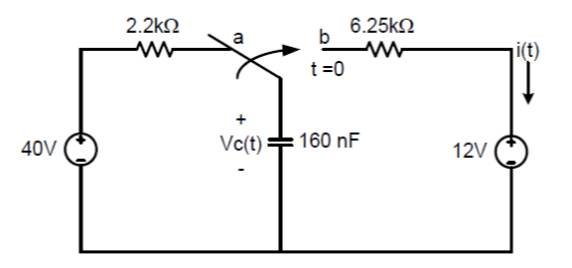
\includegraphics[width=0.7\textwidth]{Example1.jpg}
\caption{Circuit to accompany example 1}
\label{fig: Example1}
\end{figure}

\soln{6in}{
Step 1 - Find the intial value of $v_c(t)$
If we assume the the switch has been in position a for a long time (that is the circuit is in steady state), we can treat the capacitor as an open circuit and recognize that $v_c(0^-)=v_{oc}$.  Since the capacitor is an open circuit and no current flows in the loop,
\[
v_c(0^-) = 40\ V
\]
Since the capacitor voltage cannot be discontinuous we know that
\[
v_c(0^+) = 40\ V
\]

Step 2 - Find the final value of $v_c(t)$ that is find $v_c(\infty)$
Using the same logic as in step 1, it should be clear that
\[
v_c(\infty) = 12\ V
\]

Step 3 - Recall that $v_c(t)$ will have the form
\[
v_c(t) = (V_0-V_A)e^{-\frac{t}{RC}} + V_A
\]
where $V_0$ is the initial value of $v_c$ and $V_A$ is its final value; $R$ is the Thevenin resistance of the circuit for $t\ge0$ (in this case $R=6.25\ k\Omega$)

Step 4 - Plug in values to arrive at
\[
v_c(t) = 28e^{-1000t} + 12 \quad \quad t\ge0
\]
which can also be written as
\[
v_c(t) = (28e^{-1000t} + 12)u(t)
\]

Step 5 - Find $i(t)$.  We can find $i(t)$ using two methods.

Method 1 - Use Ohms law

Note that the $i(t)$ flows through the $6.25\ k\Omega$ resistor.  The voltage across the resistor is $v_c(t) -12\ V$ (write a KVL equation if necessary to see that).  This means that:
\[
i(t) = \frac{v_c(t) -12\ V}{6.25\ k\Omega}
\]
\[
i(t) = \frac{(28e^{-1000t} + 12)u(t) -12\ V}{6.25\ k\Omega} = 4.48e^{-1000t}u(t)\ mA
\]

Method 2 - Use the capacitor $i$--$v$ characteristic
\[
i(t) = -C\frac{\partial v_c(t)}{\partial t}
\]
Note the $-$ sign comes from the passive sign convention ($i(t)$ is leaving the positive terminal of the capacitor).
\[
\frac{\partial v_c(t)}{\partial t}= -28,000e^{-1000t}u(t)
\]
\[
i(t) = -160\ nF \times -28,000e^{-1000t}u(t) = 4.48e^{-1000t}u(t)\ mA
\]

The same result as Method 1!

$v(t)$ and $i(t)$ are plotted below:

\begin{figure} [h!]
\centering
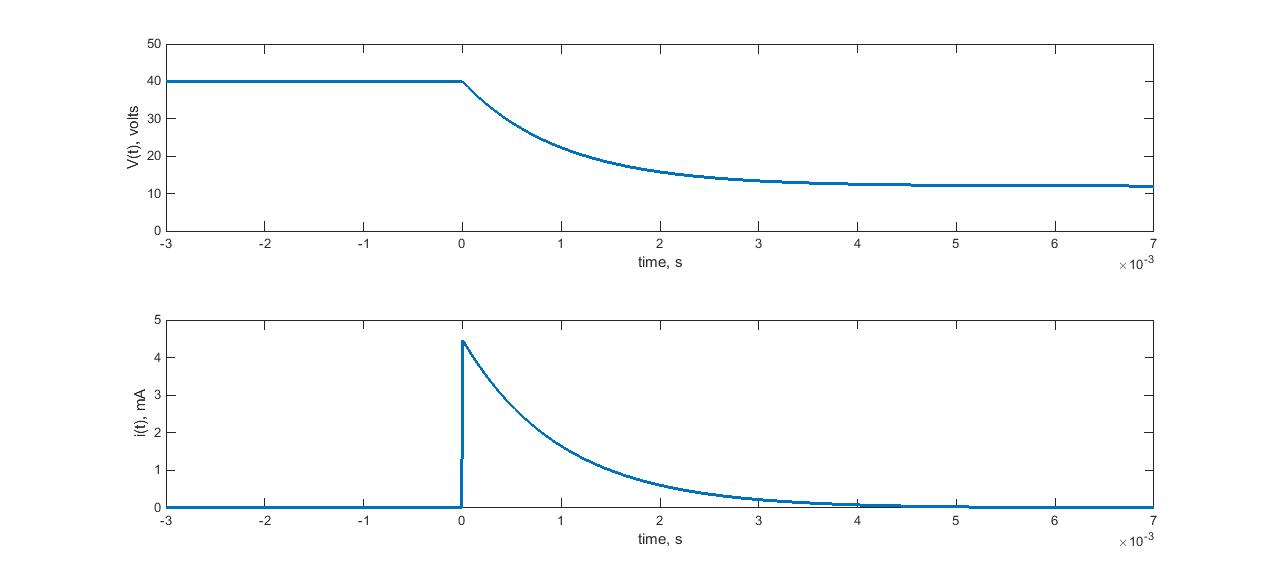
\includegraphics[width=1\textwidth]{Example1_plots.jpg}
\end{figure}
}


\newpage
\clearpage
\pagebreak

\textbf{Example 2}  -- For the circuit shown in Figure \ref{fig: Example2}, find $v_c(t)$ and $i(t)$.

\begin{figure} [h!]
\centering
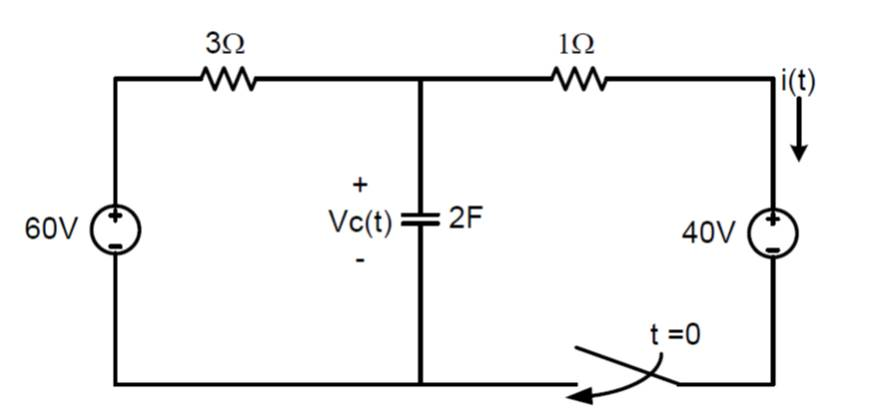
\includegraphics[width=0.7\textwidth]{Example2.jpg}
\caption{Circuit to accompany example 2}
\label{fig: Example2}
\end{figure}

I will show 2 solutions for this one....

\soln{6in}{
Solution \#1 - Use Node Voltage Analysis

We we will use the bottom node as our reference node.  For there we can write a node voltage equation for that gives the voltage across the capacitor, $v_c(t)$':
\[
\frac{v_c(t)-60}{3}+2\frac{\partial v_c(t)}{\partial t}+\frac{v_c(t)-40}{1}=0
\]
Rearranging we arrive at:
\[
\frac{\partial v_c(t)}{\partial t} +\frac{2}{3}v_c(t)= 30
\]

First we solve for the natural response, $v_{c-n}(t)$, which is the solution to
\[
\frac{\partial v_c(t)}{\partial t} +\frac{2}{3}v_c(t)=0
\]
The solution has the form
\[
v_{c-n}(t) = Ke^{-\frac{t}{RC}}
\]
It should be easy to see that $RC = \frac{3}{2}$ so the natural response is
\[
v_{c-n}(t) = Ke^{-\frac{2t}{3}}
\]
We have to wait to solve for K!  The forced response is the solution to:
\[
\frac{\partial v_{c-f}(t)}{\partial t} +\frac{2}{3}v_{c-f}(t)= 30
\]
We can re-write this as
\[
\frac{3}{2}\frac{\partial v_{c-f}(t)}{\partial t} +v_{c-f}(t)= 45
\]
One solution to this equation is to let $v_{c-f}(t) =45\ V$.  If $v_{c-f}(t)$ is constant the derivative vanishes.

Out complete solution is the sum of the natural response and the forced response
\[
v_c(t) = Ke^{-\frac{2t}{3}} + 45
\]
It should be easily seen that $v_c(0) = 60\ V$.  We can use this intial condition to find K
\[
60 = Ke^{-\frac{2\times 0}{3}} + 45
\]
Therfore $K=15$. So finally we arrive at
 \[
v_c(t) = (15e^{-\frac{2t}{3}} + 45)u(t)
\]
where the $u(t)$ is because this result is only valid for $t>0$.

By inspection of the circuit we see that
\[
i(t) = \frac{v_c(t)-40}{1\ \Omega} = (15e^{-\frac{2t}{3}} + 5)u(t)
\]
}

That was the rigourous way, now let's look at what I think is an easier way (but it does rely on a little more intuition)

\soln{6in}{
Solution 2 -- Find $v_c(0)$,  $v_c(\infty)$, and the time constant, $\tau=R_TC$; then plug into standard form of the soultion.

Just like in the first solution, $v_c(0)=60\ V$ (I hope this is realtively obvious)

What is $v_c(\infty)$?  To find this, we need to look at what the {\em final} circuit looks like; the figure below shows what the circuit looks like for $t>5\tau$.  Since the circuit has once again reached a steady state, the capacitor is effectively an open circuit.
\begin{figure} [h!]
\centering
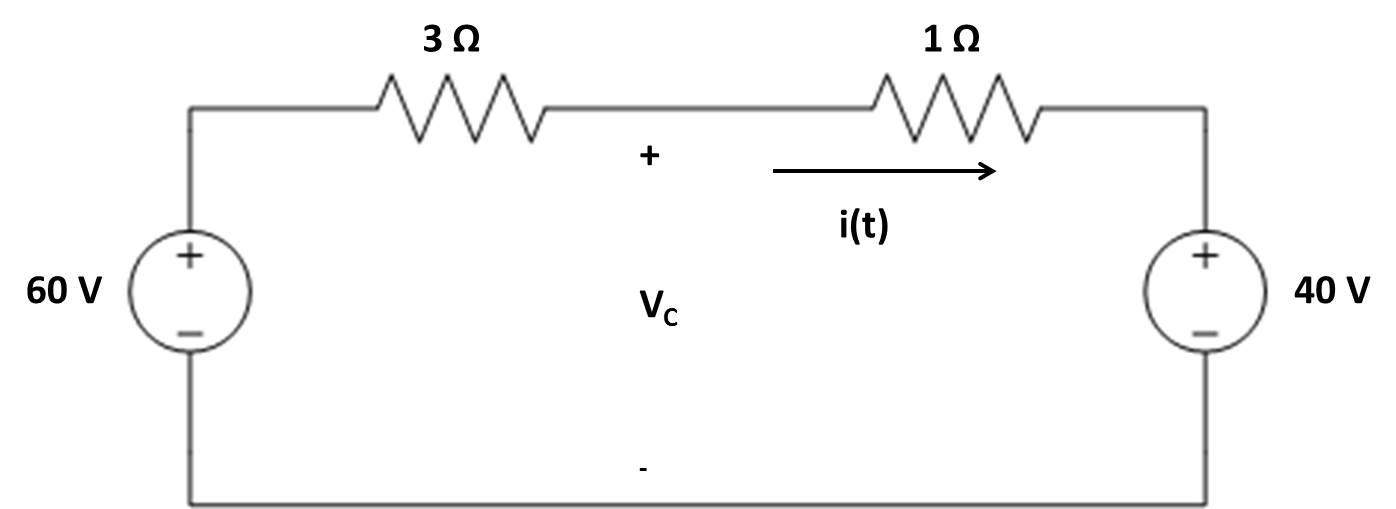
\includegraphics[width=0.7\textwidth]{Example2solnA.jpg}
\end{figure}
From this circuit it is easy to find $i(\infty)$ by writing a KVL equation for the loop
\[
60 - 3i(\infty) -1i(\infty) -40 =0
\]
\[
i(\infty) = 5A
\]
We can write a slightly different KVL equation to find $v_c(\infty)$
\[
60 - 3i(\infty) -v_c(\infty)=0
\]
Therefore
\[
v_c(\infty) = 60-15 =45\ V
\]

Next we have to find the Thevenin resistance seen by the capacitor (should be easy to find using lookback technique)
\[
R_T = 3\ \Omega||1\ \Omega = \frac{3}{4}\ \Omega
\]
From here we find $\tau$
\[
\tau =R_TC= \frac{3}{4}\ \Omega \times 2F = \frac{3}{2}s
\]
Finally recall our standard solution has the form
\[
v(t) = \left[(V_0-V_A)e^{-\frac{t}{R_TC}} + V_A\right]u(t)
\]
where $V_0 = v_c(0)$, $V_A = v_c(\infty)$.  Plugging our results in yields
\[
v(t) = \left[15e^{-\frac{2t}{3}} + 45\right]u(t)
\]

Same as solution \#1!

}

\newpage
\clearpage
\pagebreak
\section{RL Circuit Forced Response to Step Function Inputs}
Our treatment of $RL$ circuits will closely follow our treatment of RC circuits.  Our total response will still be the sum of the natural and forced resposnes but we for inductor circuits we write current equations:
\soln{0.75in}{
\[
i(t) = i_N(t) + i_F(t)
\]
}

We have to start with the differential equation for an RL circuit:
\soln{0.75in}{
\[
i(t) + \frac{L}{R}\frac{\partial i(t)}{\partial t} = I_Au(t)
\]
}
where $I_A$ is the forcing function (source).

We know from previous lessons that the natural response of an $RL$ circuit has the form:
\soln{0.75in}{
\[
i_N(t) = \left[Ke^{_\frac{R_Tt}{L}}\right]u(t)
\]
}
where $R_T$ is the Thevenin resistance of the circuit as seen by the inductor.  Also note that the time constant is $\tau = \frac{L}{R_T}$.

The forced response is the solution to
\soln{0.75in}{
\[
i_F(t) + \frac{L}{R}\frac{\partial i_F(t)}{\partial t} = I_Au(t)
\]
}
Just like for RC circuits, one obvious solution to this equation is
\soln{0.75in}{
\[
i_F(t) = I_A
\]
}

This gives us a total response of
\soln{0.75in}{
\[
i_N(t) + i_F(t) = \left[Ke^{_\frac{R_Tt}{L}}+ I_A\right]u(t)
\]
}

To find $K$ we use our initial condition ($i_(0) = I_0$)
\soln{0.75in}{
\[
K = I_0-I_A
\]
}

So our final solution looks like
\soln{0.75in}{
\[
i(t) = \left[( I_0-I_A)e^{_\frac{R_Tt}{L}}+ I_A\right]u(t)
\]
}

\newpage
\clearpage
\pagebreak

\textbf{Example 3} -- For the circuit shown in Figure \ref{fig: Example3}, find $i(t)$ for $t>0$  (notice this is equal to $i_l(t)$.
\begin{figure} [h!]
\centering
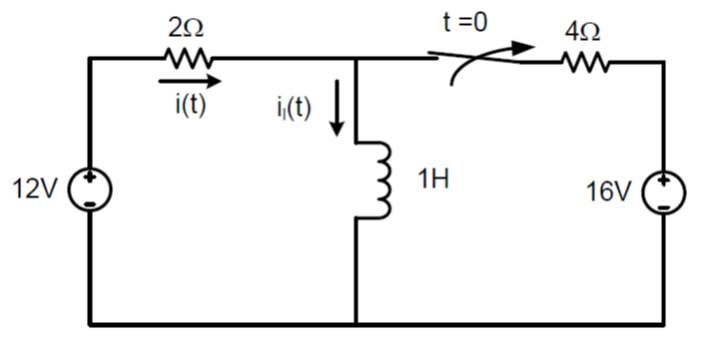
\includegraphics[width=0.7\textwidth]{Example3.jpg}
\caption{Circuit to accompany example 3}
\label{fig: Example3}
\end{figure}

\soln{6in}{
Our first step is to find the current through the inductor, $i_l$ before the switch is opened at $t=0$

If we assume the switch has been closed for a long time, the inductor looks like a short.  This makes the circuit effectively look like:
\begin{figure} [h!]
\centering
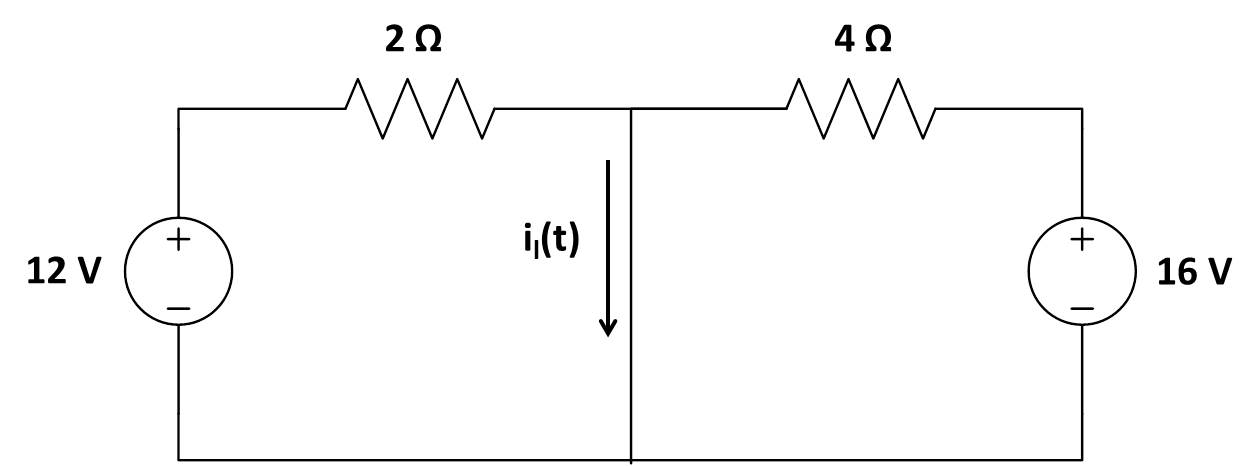
\includegraphics[width=0.7\textwidth]{Example3solnA.jpg}
\end{figure}

We can use source transformations to find $i_l(t)$.
\begin{figure} [h!]
\centering
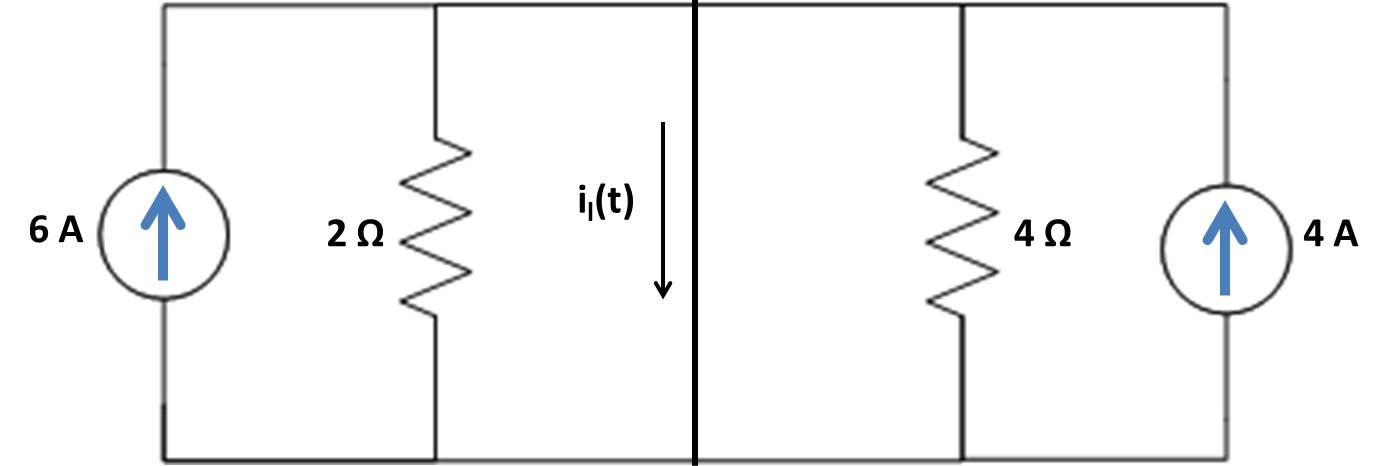
\includegraphics[width=0.7\textwidth]{Example3solnB.jpg}
\end{figure}
This figure should make it obvious that $i_l(t) = 10A$.  Remember this circuit is only valid for $t<0$.  This gives us our initial condition, $I_0 = 10\ A$

\newpage
\clearpage
\pagebreak

For $t>0$ the circuit looks like:
\begin{figure} [h!]
\centering
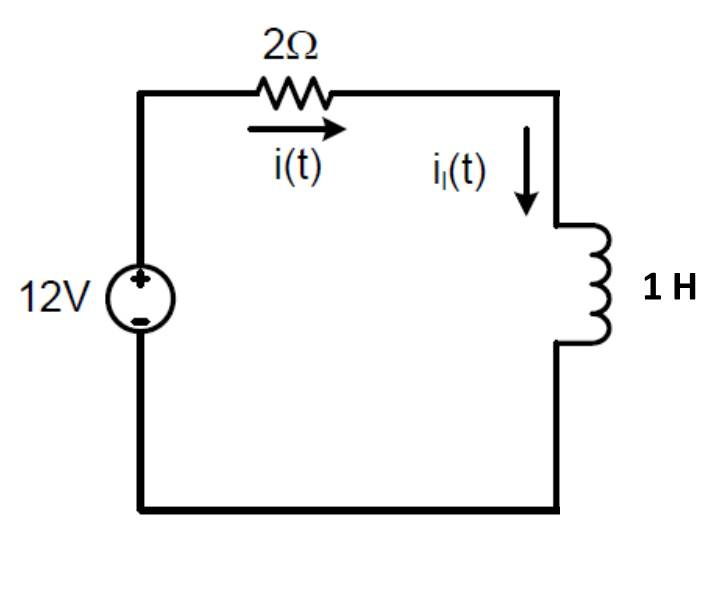
\includegraphics[width=0.4\textwidth]{Example3solnC.jpg}
\end{figure}

We can write a differential equation for this loop using KVL:
\[
12V - v_R(t) - v_L(t) = 0
\]
which using Ohms law and the $i$--$v$ characteristic of an inductor can be rewritten as
\[
12V -2i(t) - \frac{\partial i(t)}{\partial t} = 0
\]
rearranging this equation into standard form gives:
\[
i(t) +\frac{1}{2}\frac{\partial i(t)}{\partial t} = 6
\]

The natural response is easily found from what we already know
\[
i_N(t) = \left[Ke^{-2t}\right]u(t)
\]

The forced response is easily found from our differential equation:
\[
i_F(t) = 6\ A
\]

So our total response is the sum of these
\[
i(t) = \left[Ke^{-2t} + 6\right]u(t)
\]

K is found using our initial condition
\[
Ke^{-2 \times 0} + 6 =10
\]
\[
K=4
\]

Giving us a final result of
\[
i(t) = \left[4e^{-2t} + 6\right]u(t)
\]
}

\newpage
\clearpage
\pagebreak

\textbf{Example 4} -- For the circuit shown in Figure \ref{fig: Example4}, find $i_l(t)$ and $v(t)$

\begin{figure} [h!]
\centering
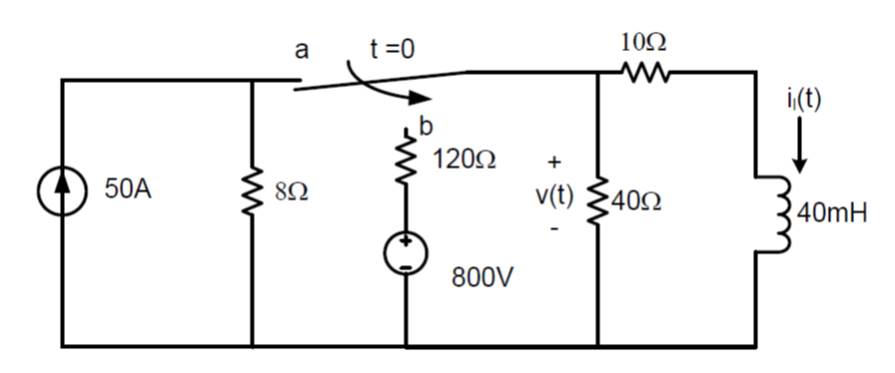
\includegraphics[width=0.7\textwidth]{Example4.jpg}
\caption{Circuit to accompany example 4}
\label{fig: Example4}
\end{figure}

\soln{6in}{
\begin{figure} [h!]
\centering
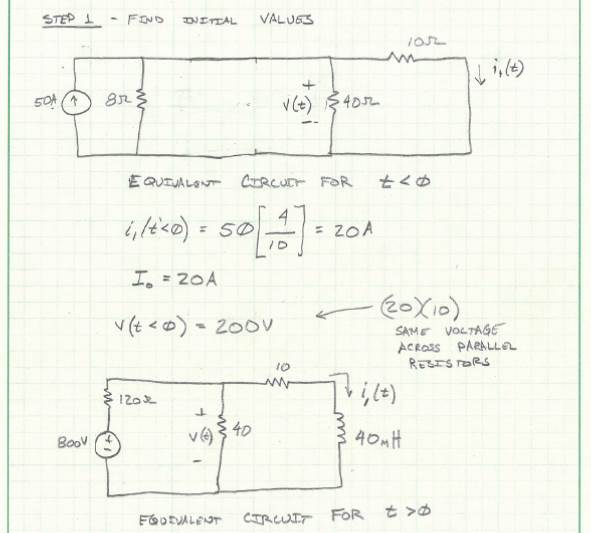
\includegraphics[width=0.9\textwidth]{Example4solnA.jpg}
\end{figure}
}

\newpage
\clearpage
\pagebreak

\soln{6in}{
\begin{figure} [h!]
\centering
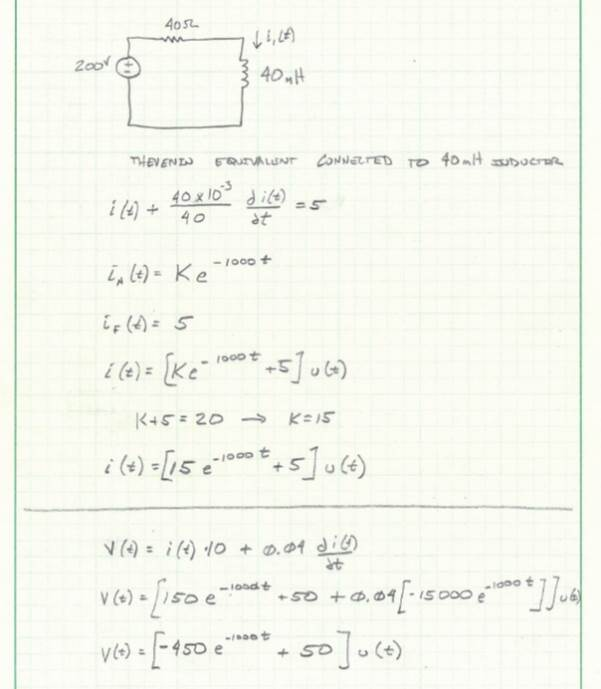
\includegraphics[width=1\textwidth]{Example4solnB.jpg}
\end{figure}
}


\newpage
\clearpage
\pagebreak

\section{Forced Response to Exponential}
The natural response is the same regardless of the form of the forcing function, so we will not go over that portion again.  What does the forced response from an exponential input look like?  It is the solution of the following equation:
\[
RC\frac{\partial v(t)}{\partial t}+v(t) = V_Ae^{-\alpha t}u(t)
\]

Like for the step function case we are going to guess a form of the forced response:
\soln{0.75in}{
\[
v_F(t) = Ae^{-\alpha t}
\]
}

If we plug this {\em solution} back into the differential equation we can solve for $A$:
\soln{3in}{
\[
RC\frac{\partial }{\partial t}Ae^{-\alpha t}+Ae^{-\alpha t} = V_Ae^{-\alpha t}u(t)
\]
\[
-RC\alpha Ae^{-\alpha t}+Ae^{-\alpha t} = V_Ae^{-\alpha t}u(t)
\]
Factor out $A$ ane $e^{-\alpha t}$
\[
A \left[1 - RC\alpha\right] = V_A
\]
Therefore:
\[
A = \frac{ V_A}{ \left[1-RC\alpha \right]}
\]

This is much easier with numbers than with variables...
}

We can add this forced response to the natural response:
\soln{1in}{
\[
v(t) = Ke^{-\frac{t}{RC}}+\frac{ V_A}{ \left[1-RC\alpha\right]}e^{-\alpha t}
\]
}

Finally, we use our initial condition to solve for the coeeficient $K$.

I have shown the derivation for an $RC$ circuit and will show and $RC$ example.  You should be able to do the development of the $RL$ circuit on your own.

\newpage
\clearpage
\pagebreak

\textbf{Example 5} -- For the circuit shown in Figure \ref{fig: Example5}, find $v_c(t)$ and $i(t)$

\begin{figure} [h!]
\centering
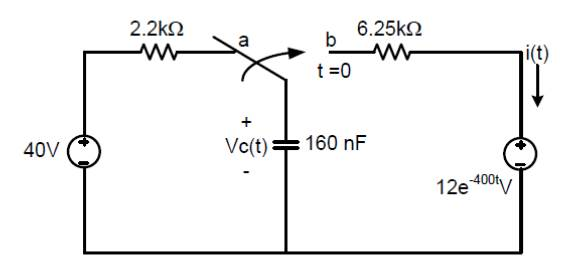
\includegraphics[width=0.7\textwidth]{Example5.jpg}
\caption{Circuit to accompany example 5}
\label{fig: Example5}
\end{figure}

\soln{6in}{
\begin{figure} [h!]
\centering
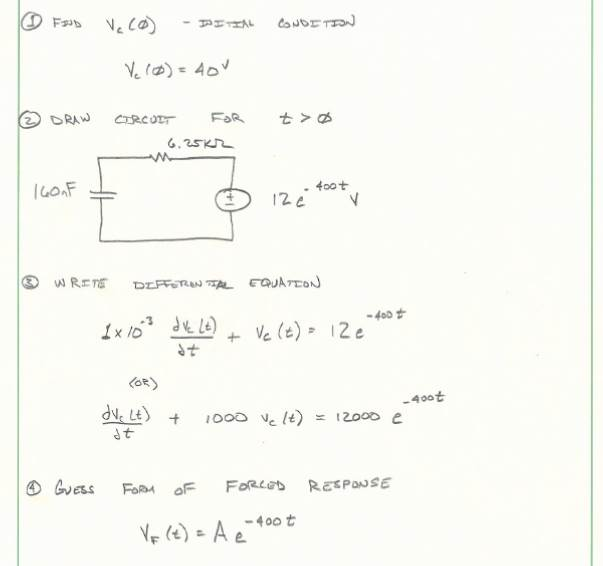
\includegraphics[width=0.9\textwidth]{Example5solnA.jpg}
\end{figure}
}

\newpage
\clearpage
\pagebreak

\soln{6in}{
\begin{figure} [h!]
\centering
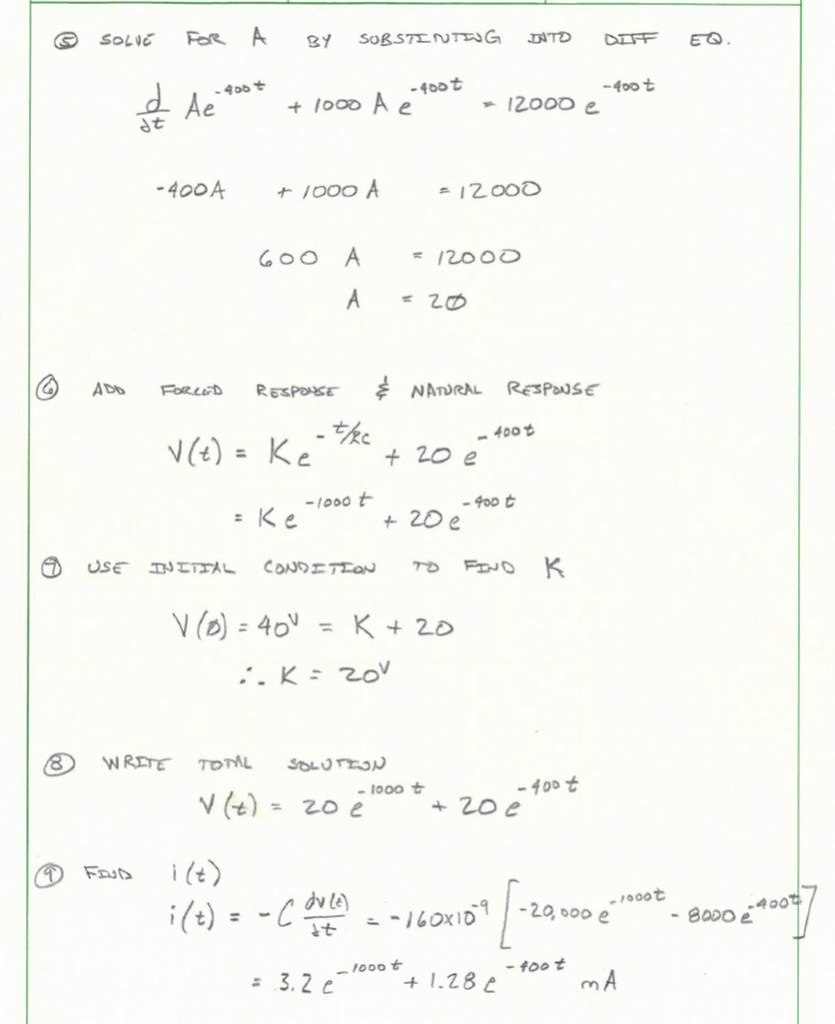
\includegraphics[width=1\textwidth]{Example5solnB.jpg}
\end{figure}
}

\newpage
\clearpage
\pagebreak

\section{Forced Response to a Sinusoid}
The natural response is the same regardless of the form of the forcing function, so we will not go over that portion again.  What does the forced response from an sinusoidal input look like?  It is the solution of the following equation:
\[
RC\frac{\partial v(t)}{\partial t}+v(t) = V_A\cos (\omega t)u(t)
\]

Like for the step function and exponential cases we are going to guess a form of the forced response:
\soln{0.75in}{
\[
v_F(t) = a\cos (\omega t) +b \sin (\omega t)
\]
}

If we plug this {\em solution} back into the differential equation we get:
\soln{3in}{
\[
RC\left[ -a\omega\sin(\omega t) + b\omega \cos(\omega t) \right] + a\cos (\omega t) +b \sin (\omega t) =V_A\cos (\omega t)
\]
Grouping $\sin$ and $\cos$ terms we get
\[
\left[bRC\omega +a \right]\cos (\omega t) + \left[-aRC\omega +b\right] \sin (\omega t)=V_A\cos (\omega t)
\]
Therefore:
\[
a = \frac{V_A}{1+(\omega RC)^2}
\]
\[
b = \frac{\omega RCV_A}{1+(\omega RC)^2}
\]

This is much easier with numbers than with variables...
}

We can add this forced response to the natural response:
\soln{1in}{
\[
v(t) = Ke^{-\frac{t}{RC}}+\frac{V_A}{1+(\omega RC)^2}\cos (\omega t) +\frac{\omega RCV_A}{1+(\omega RC)^2} \sin (\omega t)
\]
}

Finally, we use our initial condition to solve for the coeeficient $K$.

I have shown the derivation for an $RC$ circuit and will show and $RC$ example.  You should be able to do the development of the $RL$ circuit on your own.

\newpage
\clearpage
\pagebreak

\textbf{Example 5} -- For the circuit shown in Figure \ref{fig: Example5}, find $v_c(t)$ and $i(t)$

\begin{figure} [h!]
\centering
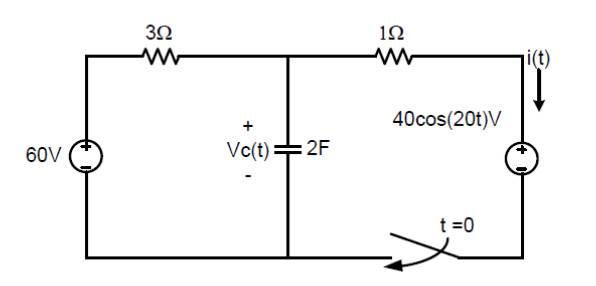
\includegraphics[width=0.7\textwidth]{Example6.jpg}
\caption{Circuit to accompany example 5}
\label{fig: Example5}
\end{figure}

\soln{6in}{
\begin{figure} [h!]
\centering
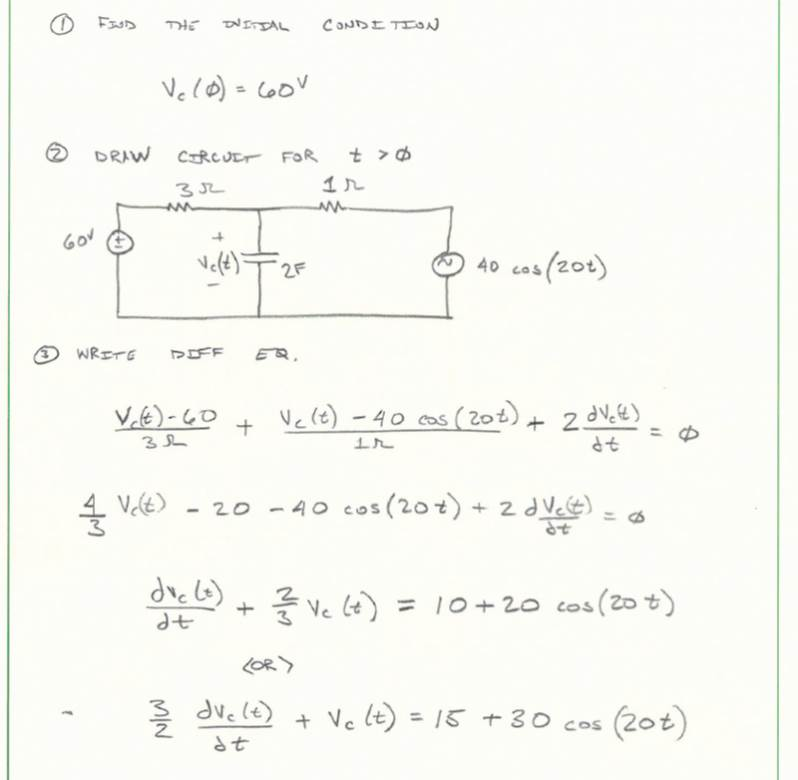
\includegraphics[width=0.9\textwidth]{Example6solnA.jpg}
\end{figure}
}

\newpage
\clearpage
\pagebreak

\soln{6in}{
\begin{figure} [h!]
\centering
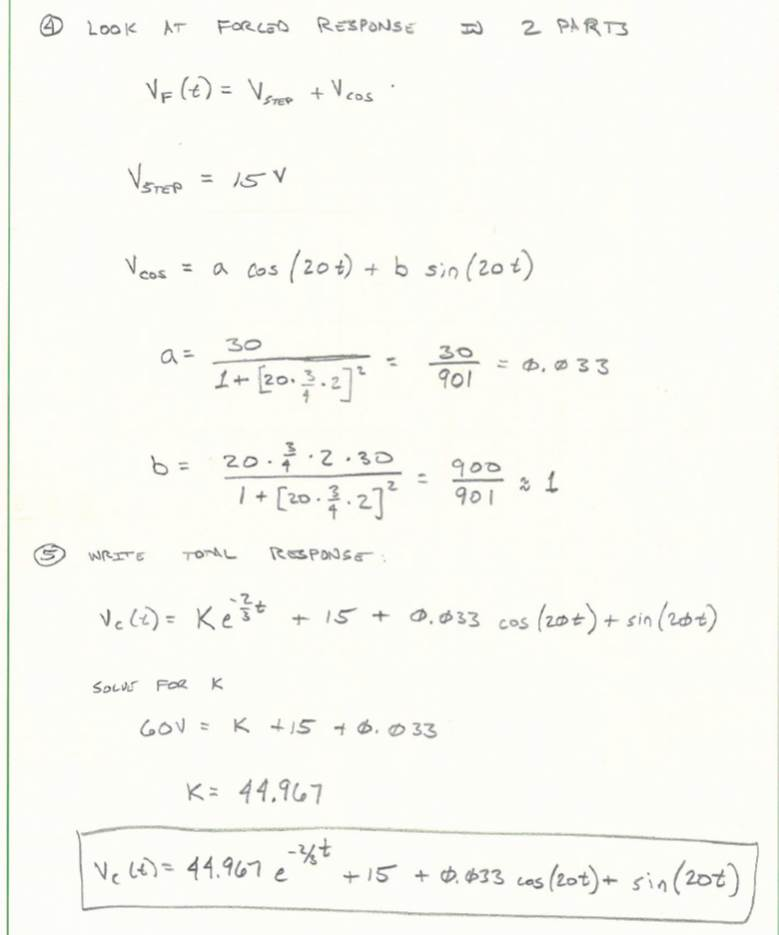
\includegraphics[width=1\textwidth]{Example6solnB.jpg}
\end{figure}
}


\newpage
\clearpage
\pagebreak

\newpage
\clearpage
\pagebreak

\newpage
\clearpage
\pagebreak

\end{document}


% Equation Array Example Code
%\begin
%{eqnarray}
%P_R &=& i_R^2R \nonumber \\
%P_R &=& (100\ mA)^2 \times 100\ \Omega \nonumber \\
%P_R &=& (100 \times 10^{-3}\ A)^2 \times 100\ \Omega \\
%P_R &=& 10000 \times 10^{-6}\ A^2  \times 100\ \Omega \nonumber \\
%P_R &=& 1\ W  \nonumber
%\end{eqnarray}

% Figure Example Code
%\begin{figure} [h!]
%\centering
%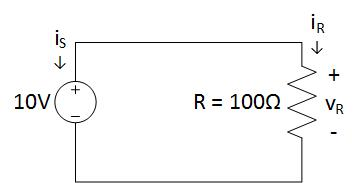
\includegraphics[width=0.5\textwidth]{OhmsLawExampleSolution.jpg}
%\caption{Ohm's Law example circuit}
%\label{fig: OhmsLawExampleSolution}
%\end{figure}

%Table Example Code
%\begin{table}[h]
%\centering
%\begin{tabular}{|l|c|c|}
%\hline
%Prefix & Abbreviation & Value \\
%\hline \hline
%Giga & $G$ & $10^9$ \\
%Mega & $M$ & $10^6$ \\
%Kilo & $k$ & $10^3$ \\
%\hline
%milli & $m$ & $10^{-3}$ \\
%micro & $\mu$ & $10^{-6}$ \\
%nano & $n$ & $10^{-9}$ \\
%pico & $p$ & $10^{-12}$ \\
%\hline
%\end{tabular}
%\caption{Engineering prefixes and values}
%\label{tab: Eng Prefixes}
%\end{table}
